\begin{tikzpicture}

	\draw [thick, gray, <->] (10,2) -- (10,7)      % draw y-axis line
	node [above, black] {$\nabla w_2$};              % add label for y-axis
	%node [below,black]{$-y$};
	\draw [thick, gray, <->] (7,4.5) -- (13,4.5)      % draw x-axis line
	node [right, black] {$\nabla w_1$};  
	\draw[->,draw=black,ultra thick](10,4.5)--(11.5,2.6);
	\only<2-8>{
		\draw[->,draw=green!100,thick](10,4.5) -- (10.6,5.3);}
	\only<3-8>{
		\draw[->,draw=blue,thick](10.6,5.3)--(10.6,4.5);}
	\only<4-8>{
		\draw[->,draw=red,thick](10.6,4.5)--(11,4.5);}
	\only<5-8>{
		\draw[->,draw=blue,thick](11,4.5)--(11,3.8);}
	\only<6-8>{
		\draw[->,draw=red,thick](11,3.8)--(11.5,3.8);}
	\only<2-8>{
		\node(label1) at (11.5,6.6){starting from this};
		\node(label2) at (11.9,6.2){initial position};
		\node(label3) at (12.3,5.8){only way to reach it};
		\node(label4) at (12.6,5.4){is by taking a \textcolor{red}{zigzag} path};
		\draw[->,draw=black,thick](10.5,6.45)--(10.5,5.35);
	}
	
	\only<7-8>{    \draw[->,draw=blue,thick](11.5,3.8)--(11.5,2.6);}
	
\end{tikzpicture}      